
\chapter{原子轨道}


\section{单电子体系(类氢原子)波函数求解}



\[
    \left[ \frac{1}{r^2} \frac{\partial}{\partial r} \left( r ^2 \frac{\partial}{\partial r} \right) + \frac{1}{r^2 \sin \theta} \frac{\partial}{\partial \theta} \sin \theta \frac{\partial}{\partial \theta} + \frac{1}{r^2 \sin ^2 \theta} \frac{\partial^2}{\partial \phi^2} \right]   \psi (r, \theta, \phi) + \frac{2m}{\hbar}\left[ E + \frac{Ze^2}{4\pi \epsilon_0 r }  \right] \psi(r, \theta, \phi) = 0
\]

分离变量

\[
   \psi = R(r) \cdot Y(\theta, \phi)  
\]

\[
    \frac{Y}{r^2} \frac{\partial}{\partial r} \left( r^2 \frac{\partial R}{\partial r } \right) + \frac{R}{r^2 \sin \theta} \frac{\partial }{\partial \theta} \left(\sin \theta \frac{\partial Y}{\partial \theta} \right) + \frac{R}{r^2 \sin ^2 \theta} \frac{\partial^2 Y}{\partial \phi^2} + \frac{2m}{\hbar}\left[ E + \frac{Ze^2}{4\pi \epsilon_0 r }  \right] RY = 0
\]

两边同时乘以 $\frac{r^2}{R \cdot Y}$

\[
    \frac{1}{R} \frac{\partial}{\partial r} \left( r^2 \frac{\partial R}{\partial r} \right) + \frac{1}{Y \sin \theta} \frac{\partial }{\partial \theta} \left( \sin \theta \frac{\partial Y}{\partial \theta} \right) + \frac{1}{Y \sin ^2 \theta} \frac{\partial ^2 Y}{\partial \phi ^2} + \frac{2m}{\hbar}\left[ E + \frac{Ze^2}{4\pi \epsilon_0 r }  \right] r^2 = 0 
\]

现在整个方程就可以分为一个和角度有关,一个和长度有关。我们可以把与角度、长度有关的量分别提出来。

\[
    \frac{1}{R} \frac{\partial}{\partial r} \left( r^2 \frac{\partial R}{\partial r} \right) + \frac{2m}{\hbar}\left[ E + \frac{Ze^2}{4\pi \epsilon_0 r }  \right] r^2 = k
\]

\[
    \frac{1}{Y \sin \theta} \frac{\partial}{\partial \theta} \left( \sin \theta \frac{\partial Y}{\partial \theta} \right) + \frac{1}{Y \sin ^2 \theta} \frac{\partial ^2 Y}{\partial \phi ^2} = -k 
\]

先看下面这个方程,我们需要继续分离两个角度,也就是$\theta$和$\phi$

\[
    Y = \Theta(\theta) \cdot \Phi(\phi)  
\]

\[
    - \frac{1}{\Theta \Phi} \left[ \frac{\Phi}{ \sin \theta} \frac{\partial}{\partial \theta} \left( \sin \theta \frac{\partial \Theta}{\partial \theta} \right) + \frac{\Theta}{ \sin ^2 \theta} \frac{\partial ^2 \Phi}{\partial \phi ^2} \right] = k
\]

\[
    - \frac{1}{\Theta} \frac{1}{ \sin \theta} \frac{\partial}{\partial \theta} \left( \sin \theta \frac{\partial \Theta}{\partial \theta} \right) - \frac{1}{ \sin ^2 \theta \Phi} \frac{\partial ^2 \Phi}{\partial \phi ^2} = k
\]

为了让两边一个只有$\theta$,一个只有$\phi$,同时乘以$\sin ^2   \theta$

\[
    - \frac{1}{\Theta}  \sin \theta \frac{\partial}{\partial \theta} \left( \sin \theta \frac{\partial \Theta}{\partial \theta} \right) - \frac{1}{\Phi} \frac{\partial ^2 \Phi}{\partial \phi ^2} = k \sin ^2 \theta
\]

移项

\[
    -\frac{1}{\Phi} \frac{\partial ^2 \Phi}{\partial \phi ^2} = k \sin ^2 \theta  + \frac{\sin \theta}{\Theta}   \frac{\partial}{\partial \theta} \left( \sin \theta \frac{\partial \Theta}{\partial \theta} \right)
\]

两边必须同时等于一个常数 

\[
     - \frac{1}{\Phi} \frac{\partial ^2 \Phi}{\partial \phi ^2} = m^2
\]

这个方程也就是 $\Phi$ 方程

\[
    \frac{\partial ^2 \Phi}{\partial \phi ^2} + m^2 \Phi  = 0
\]

显然,设$\Phi = A e^{a \phi}$ 

\[
    a^2 e^{a \phi} + m^2 e^{a \phi} = 0
\]

\[
    a = \pm im  
\]

\[
    \Phi = \begin{cases}
        Ae^{im\phi} & = A( \cos im\phi + i \sin im \phi)  \\
        Ae^{-im\phi} & =  A( \cos im\phi - i \sin im \phi) \\
    \end{cases}  
\]

归一化条件:


\[
    \int_0^{2\pi} A^2 d\phi = 1 
\] 

\[
    A = \frac{1}{\sqrt{2\pi}}  
\]

\[
    \Phi = \frac{1}{\sqrt{2\pi}} e ^{im\phi}  
\]

\[
    e^{im\phi} = e^{im\phi} \cdot e^{im2\pi}  
\]

\[
    e^{im 2\pi} = 1  \qquad \mbox{m只能取整数} m \in Z
\]


\section{量子数的物理意义}

\subsection{主量子数$n$}

\begin{align*}
    E_n &= - \frac{me^4}{8 \pi \epsilon_0^2 h^2} \frac{Z^2}{n^2} \\ 
    &= - 13.6 \frac{Z^2}{n^2} (\mathrm{eV})\\
\end{align*}

$n$的取值决定能量的高低。能量最低时,依然不为0,具有零点能效应。这里的``零点能''指的是$n = 1$的取值,由于一些历史原因,被称为零点能。

\subsection{角量子数$l$}

\begin{equation*}
    \frac{2m r^2}{\hbar ^2} = l \cdot (l + 1)
\end{equation*}

\begin{equation*}
    \frac{8 \pi^2 m r ^2}{h^2} T_{\mbox{转}} = l \cdot (l + 1)
\end{equation*}

\begin{equation*}
    T_{\mbox{转}} = \frac{l \cdot (l + 1)}{8 \pi^2 I}
\end{equation*}

\begin{equation*}
    \mathbf{l} = \sqrt{l(l + 1)}\hbar
\end{equation*}


$l$决定原子轨道的形状、电子云的形状。

\subsection{磁量子数$m$}

\begin{align*}
    \hat{M}_z &= -i\hbar \frac{\partial}{\partial \phi} \psi(r, \theta, \phi) \\ 
    &= - R(r) \Theta(\theta) i \hbar \frac{\partial}{\partial \phi} \left( \frac{1}{\sqrt{2\pi}} e^{im\phi} \right) \\
    &= R(r) \Theta(\theta) \hbar m \left( \frac{1}{\sqrt{2\pi}} e^{im\phi} \right)
\end{align*}

\begin{equation*}
    \mathbf{l}_z = m\hbar = m\frac{h}{2\pi}
\end{equation*}

在磁场中,要考察电子运动产生的磁矩,需要应用磁量子数。

$m$可以决定$M_z$、$\mu_{z}$,原子轨道和电子云的取向。



\begin{align*}
    \hat{M}_z \cdot \psi (r, \theta, \phi) &= -i \hbar R(r) \Theta(\theta) \frac{\partial}{\partial \phi} \sqrt{\frac{1}{\pi}} \cos \phi  \\ 
    &= \cdots \times \sin \phi \\ 
    &\neq \cdots \times \phi(r, \theta, \phi)
\end{align*}


注意 
\begin{enumerate}
    \item $s$轨道没有角动量量子化的问题
\end{enumerate}

\subsubsection{磁矩}

\begin{equation*}
    \hat{\mu} = -\frac{e}{2m_e} \hat{M}
\end{equation*}

电子绕核运动的磁矩

\begin{equation*}
    |\mu| = \left\lvert -\frac{e}{2m_e} \hat{M} \right\rvert
\end{equation*}

玻尔磁子 $\mu_B = \frac{e\hbar}{2m_e}$

\begin{equation*}
    |\mu| = \sqrt{l(l + 1)} \mu_B
\end{equation*}


\subsection{自旋量子数$m_s$}

电子自旋 $s = \frac{1}{2}$ 


\begin{align*}
    M_s &= \sqrt{\frac{1}{2} \cdot \left( 1 + \frac{1}{2} \right)} \cdot \hbar \\ 
    &= \frac{\sqrt{3}}{2} \hbar
\end{align*}


\begin{align*}
    M_{s_z} = m_s \hbar (\pm \frac{1}{2})
\end{align*}


\begin{align*}
    \mu_{s_z} &= \pm \mu_B \\
    &= \pm \frac{e\hbar}{2m_e} \\ 
    &= -\frac{e}{m_e} \hbar (\mp \frac{1}{2}) \\ 
    &= -\frac{e}{m_e} M_{s_z} 
\end{align*}

\begin{align*}
    |u_s| &= -\frac{e}{m_e} \cdot M_s \\ 
    &= \sqrt{3} \mu_B
\end{align*}

$\psi_{n,l,m,m_s}$ 轨道波函数



\subsubsection{赛曼效应}

$\psi(1, 0, 0)$轨道,$\psi(2, 1, \pm 1, 0)$轨道算能量差,由于m有三种取值,导致角动量的方向是量子化的,方向的量子化导致绕核运动产生的磁矩是量子化的。三种量子化产生的磁矩使得能量有升高有降低。本来固定能量差的谱线分为了三条。


\section{波函数与轨道}

三个量子数一定后,可以确定一个“原子轨道”,这个轨道并不是真正意义上的轨道,而是想象出来的,描述电子运动状态的概念,即$\psi(n, l, m)$。


\subsection{简并轨道}


所有能量相同的轨道称为简并轨道,简并轨道的个数为$n^2$个。


\subsection{轨道表示}

\begin{table}[H]
    \centering
    \begin{tabular}{ll}
        \toprule
        l & 符号 \\ 
        \midrule
        0 & s \\
        1 & p \\ 
        2 & d \\
        3 & f \\
        \bottomrule
    \end{tabular}

\end{table}
m的取值表示为$x, y, z, z^2, x^2 - y^2$。

\begin{align*}
    \psi_{210} &= \frac{1}{4 \sqrt{2 \pi}} \left( \frac{Z}{a_0} \right)^{\frac{3}{2}} \rho \cdot e^{-\frac{\rho}{2}} \cdot \cos \theta \\ 
    &= \dots e^{-\frac{\rho}{2}} r \cos \theta \\
    &= f(r) r \cdot \cos \theta \\
    &= f(r) z
\end{align*}


\subsection{轨道的形状}

\subsubsection{$s$轨道}

\begin{equation*}
    Y = \sqrt{\frac{1}{4\pi}}
\end{equation*}

如图\ref{fig:s_orbital}所示,是一个球形。

\begin{figure}[h]
    \centering
    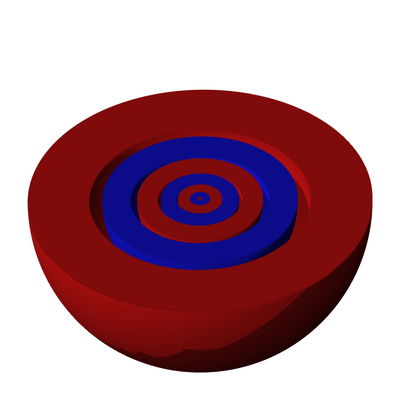
\includegraphics[width=0.5\textwidth]{images/400px-S7M0.png}
    \caption{$7s$轨道的图像}
    \label{fig:s_orbital}
\end{figure}

\subsubsection{$p$轨道}

\begin{equation*}
    Y = \sqrt{\frac{3}{4\pi}} \cos \theta
\end{equation*}

图\ref{fig:p_orbital}展示了$p$轨道的情况

\begin{figure}[h]
    \centering
    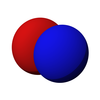
\includegraphics[width=0.5\textwidth]{images/P2y.png}
    \caption{由左而右为2p、3p、4p、5p、6p轨道的立体模型}
    \label{fig:p_orbital}
\end{figure}



\subsubsection{图像的特点}

\begin{enumerate}
    \item $l,m$不同,$n$相同,$Y$相同,$n$与图形无关
    \item $l$不同,$Y$图的形状不同 $l$决定图像的形状
    \item $m$决定$Y$图的伸展方向,决定图像取向
\end{enumerate}
